\documentclass[journal,a4paper,10pt]{IEEEtran}

\usepackage{amsmath,amssymb,amsfonts}
\usepackage{algorithm}
\usepackage{algpseudocode}
\usepackage{booktabs}
\usepackage{graphicx}
\usepackage{cite}
\usepackage{url}
\usepackage{bm}
\usepackage{xcolor}
\usepackage{tikz}
\usepackage{multirow}
\usetikzlibrary{arrows.meta,positioning,shapes.geometric,fit,calc,decorations.pathreplacing}
\graphicspath{{current/}}

\DeclareMathOperator*{\argmax}{arg\,max}
\newcommand{\R}{\mathbb{R}}
\newcommand{\E}{\mathbb{E}}

\begin{document}

\title{Efficient Resource Allocation and Payment Scheme for 5G-based Healthcare Networks}

\author{Shubham~Kumar and Satendra~Kumar%
\thanks{The authors are with the Department of Computer Science and Engineering, Indian Institute of Technology Patna, Bihta, Bihar 801106, India.}}

\maketitle

\begin{abstract}
We treat 5G healthcare as a two-sided market in which healthcare service providers (HSPs) buy uplink data rate from cellular base stations (BSs). Social welfare is maximized by an iterative allocation-and-pricing rule that is incentive compatible, individually rational, weakly budget-balanced, and economically efficient. This paper makes \emph{preference} \(\rho_{wk}\) dynamic: a bidirectional LSTM forecasts HR, SpO\(_2\), blood pressure and temperature at \(5/10/15\)\,min horizons, a NEWS2-inspired fusion produces a per-user criticality \(c_n\in[0,1]\), and \(\rho_{wk}\) is the max-normalized criticality mass on each coverage set \(B_{wk}\). Reluctance \(\omega_{kw}\) is held constant on the \(W=2\), \(K=3\) topology from a one-shot radio-geometry map (cell load, RSRP, backhaul, native-user QoS, interference). Experiments use the open eICU-CRD Demo (\(N=1821\) stays). Users are split at random into two competing buyers (HSP1, HSP2). With \(r_k^{\max}=5\)\,Mbps per cell the market clears at welfare \(10.65\) and total rate \(15.01\)\,Mbps; the LSTM attains test vital MAE \(2.28\) and risk accuracy \(80.7\%\).
\end{abstract}

\begin{IEEEkeywords}
5G healthcare, WBAN, double auction, bidirectional LSTM, dynamic preference, reluctance, eICU-CRD, KKT, IoMT.
\end{IEEEkeywords}

\section{Introduction}
\label{sec:intro}

Wireless body-area networks (WBANs) stream heterogeneous physiological data to healthcare service providers (HSPs) through cellular base stations (BSs) owned by competing cellular network providers (CNPs). Advanced e-health applications---wireless patient monitoring, tele-healthcare, ambient assisted living---require medical-grade QoS: frequent uplink of high-volume raw data at low latency. The radio resource of each BS is finite and already shared with native mobile users. HSPs therefore wish to buy as much uplink as their most critical patients need; BSs wish to sell only when the compensation covers the degradation inflicted on native traffic. We model this conflict as a \emph{two-sided market} and solve it with an iterative double auction conducted by a third-party entity (TPE). HSPs (buyers) and BSs (sellers) submit bids without revealing their private utilities; the TPE announces allocation and pricing rules that induce truthful bidding and converge to the social-welfare optimum of a strictly concave program (OPT1), implemented in practice as a bid-parameterized surrogate (OPT2).

Two scalars encode the \emph{identity} of each (HSP, BS) pair:
\begin{itemize}
  \item \(\rho_{wk}\in[0,1]\): preference of HSP \(w\) for BS \(k\), driven by how many of \(w\)'s \emph{critical} subscribers sit under \(k\);
  \item \(\omega_{kw}\in[0,1]\): reluctance of BS \(k\) to serve HSP \(w\), a per-cell cost scale. This paper holds \(\omega\) constant from one radio-geometry snapshot.
\end{itemize}
Both are private. The auction never needs their numerical values---it elicits them indirectly through bids---but the \emph{true} social welfare that the auction is trying to hit is exactly the welfare generated by those parameters. If \(\rho_{wk}\) is stale, the market clears the wrong demand; if \(\omega_{kw}\) is stale, it clears the wrong supply cost.

In a smart IoMT deployment preference is not a static census. Vitals are a time series, so a patient who is stable now may decompensate within minutes, and URLLC slices must be reserved \emph{before} that event. This paper therefore \emph{models} dynamic preference: a bidirectional LSTM forecasts vital signs, a NEWS2-inspired fusion yields a per-user criticality \(c_n(t)\in[0,1]\), and \(\rho_{wk}(t)\) is rebuilt from the predicted criticality mass on each coverage set \(B_{wk}\). Reluctance is held constant during the inner dual loop and across this experiment, using one radio-geometry snapshot on the same association map. The inner auction (OPT1/OPT2, KKT stationarity, dual updates, and the associated economic properties) is unchanged; only the private preference that enters the buyer utility is generated from data.

Section~\ref{sec:base} states the market problem. Section~\ref{sec:why-dyn} explains why \(\rho_{wk}\) must be dynamic. Section~\ref{sec:lstm} specifies the LSTM--fusion--aggregation pipeline. Section~\ref{sec:omega-impl} records the constant reluctance used here. Section~\ref{sec:setup} lists the constants used in the prototype. Section~\ref{sec:results} reports the \(W=2\), \(K=3\) eICU experiment. Section~\ref{sec:ext} outlines a GNN extension. Section~\ref{sec:conc} concludes.

\section{The Base Problem}
\label{sec:base}

We follow the notation below so that dynamic preference and reluctance can be substituted into the auction without rewriting the allocation rule.

\subsection{Market}
Let \(\mathcal{W}=\{1,\ldots,W\}\) be the set of HSPs and \(\mathcal{K}=\{1,\ldots,K\}\) the set of BSs (one per CNP in the region). Each WBAN user is subscribed to exactly one HSP and associated to a serving BS. Write \(B_{wk}\) for the set of users of HSP \(w\) that currently reside in the coverage of BS \(k\). HSP \(w\) requests an uplink rate \(d_{wk}\ge 0\) from BS \(k\); BS \(k\) offers \(r_{kw}\ge 0\) to HSP \(w\). Market clearing requires \(d_{wk}=r_{kw}\). Vectors are \(\mathbf{d}_w=(d_{wk}:k\in\mathcal{K})\) and \(\mathbf{r}_k=(r_{kw}:w\in\mathcal{W})\).

\subsection{Preference, reluctance, and welfare}
The HSP utility \(S_{wk}(\rho_{wk},\mathbf{d}_w)\) is increasing in preference and strictly concave increasing in rate:
\begin{equation}
  \nabla_{\rho_{wk}} S_{wk}\ge 0,\qquad
  \nabla_{\mathbf{d}_w} S_{wk}>0,\qquad
  \nabla^2_{\mathbf{d}_w} S_{wk}\prec 0.
  \label{eq:hsp-shape}
\end{equation}
The BS cost \(T_{kw}(\omega_{kw},\mathbf{r}_k)\) is increasing in reluctance and strictly convex increasing in assigned rate:
\begin{equation}
  \nabla_{\omega_{kw}} T_{kw}\ge 0,\qquad
  \nabla_{\mathbf{r}_k} T_{kw}>0,\qquad
  \nabla^2_{\mathbf{r}_k} T_{kw}\succ 0.
  \label{eq:bs-shape}
\end{equation}
Aggregate welfare is the TPE's objective (OPT1):
\begin{align}
  \max_{\mathbf{D},\mathbf{R}}
  &\quad \sum_{w\in\mathcal{W}} S_w(\mathbf{d}_w)
     - \sum_{k\in\mathcal{K}} T_k(\mathbf{r}_k)
     \label{eq:opt1}\\
  \text{s.t.}
  &\quad \sum_{w} r_{kw}\le r_k^{\max},\quad
        r_{kw}\ge d_{wk},\quad
        d_{wk},r_{kw}\ge 0.
        \nonumber
\end{align}
Under Slater's condition the KKT system is necessary and sufficient. Writing \(\lambda_k\) for the capacity multiplier and \(\mu_{wk}\) for the clearing multiplier,
\begin{align}
  \frac{\partial S_w}{\partial d_{wk}}-\mu_{wk}^{\mathrm{opt}}&=0,
  \label{eq:kkt-hsp}\\
  \frac{\partial T_k}{\partial r_{kw}}-\mu_{wk}^{\mathrm{opt}}+\lambda_k^{\mathrm{opt}}&=0,
  \label{eq:kkt-bs}\\
  r_{kw}^{\mathrm{opt}}=d_{wk}^{\mathrm{opt}},&\quad
  \lambda_k^{\mathrm{opt}}\Bigl(\sum_w r_{kw}^{\mathrm{opt}}-r_k^{\max}\Bigr)=0.
  \nonumber
\end{align}
Because \(S_w\) and \(T_k\) are \emph{private}, the TPE cannot solve OPT1 directly. It instead runs OPT2 on reported bids \(\varrho_{wk}\ge 0\) (HSP) and \(\zeta_{kw}\ge 0\) (BS),
\begin{equation}
  \max_{\mathbf{D},\mathbf{R}}
  \sum_{w,k}\varrho_{wk}\ln d_{wk}
  -\sum_{k,w}\zeta_{kw}\frac{r_{kw}^2}{2}
  \label{eq:opt2}
\end{equation}
subject to the same constraints. The resulting allocation rule
\begin{equation}
  \tilde d_{wk}=\frac{\varrho_{wk}}{\tilde\mu_{wk}},\qquad
  \tilde r_{kw}=\frac{\tilde\mu_{wk}-\tilde\lambda_k}{\zeta_{kw}}
  \label{eq:alloc}
\end{equation}
coincides with OPT1 whenever agents bid
\begin{equation}
  \varrho_{wk}=\tilde d_{wk}\,\frac{\partial S_w}{\partial d_{wk}},
  \qquad
  \zeta_{kw}=\frac{1}{\tilde r_{kw}}\,\frac{\partial T_k}{\partial r_{kw}}.
  \label{eq:truthful-bids}
\end{equation}
Pricing \(\Gamma_w(\boldsymbol{\varrho}_w)=\sum_k\varrho_{wk}\) (HSP pays its bid) and the corresponding BS incentive \(\Upsilon_k\) make~\eqref{eq:truthful-bids} a best response. Dual variables are updated by sub-gradient descent; the iteration is individually rational, incentive compatible, weakly budget-balanced, and economically efficient.

\paragraph{What the auction does \emph{not} do.}
It does not invent \(\rho_{wk}\) or \(\omega_{kw}\). Those parameters live \emph{inside} \(S_w\) and \(T_k\). Truthful bids~\eqref{eq:truthful-bids} track the \emph{current} gradients of those functions. If the HSP's true preference has moved and the HSP still bids as if \(\rho_{wk}\) were yesterday's value, the market is incentive compatible with respect to a \emph{wrong} utility, and the ``social optimum'' is the optimum of a stale world.

\section{Why Preference Must Be Dynamic}
\label{sec:why-dyn}

\subsection{What \(\rho_{wk}\) means}
Preference \(\rho_{wk}\) is a private score in \([0,1]\) that depends on the number of critical users present in the coverage range of BS \(k\). Formally one may write a static census
\begin{equation}
  \rho_{wk}^{\mathrm{stat}}
  \;=\;
  f\bigl(\lvert\{n\in B_{wk}: n\text{ is labelled critical}\}\rvert\bigr).
  \label{eq:rho-static}
\end{equation}
Three modelling choices are implicit: criticality is a \emph{binary} tag; it is \emph{observed now}; and only the \emph{count} (not the severity mix, not the near-future trajectory) matters.

\subsection{Why that object is not enough for a smart system}
\paragraph{Criticality is a process, not a flag.}
A NEWS2-style score~\cite{royal2017news2} is a function of HR, SpO\(_2\), blood pressure and temperature. Those signals are autocorrelated. A patient with SpO\(_2=94\%\) and a downward drift is not equivalent to one with SpO\(_2=94\%\) and a stable history. A static count of ``currently abnormal'' users therefore under-provisions the HSP that is about to absorb a cluster of decompensations.

\paragraph{The radio decision is earlier than the clinical event.}
URLLC / mMTC slices are reserved on a duty cycle of seconds to minutes. If \(\rho_{wk}\) jumps only \emph{after} a fall or a desaturation, the auction grants extra \(d_{wk}\) too late. A multi-horizon forecast \(\hat{\mathbf{v}}_n(t+\tau)\), \(\tau\in\{5,10,15\}\)\,min, lets \(\rho_{wk}(t)\) rise \emph{in anticipation}.

\paragraph{Preference is a coverage-set statistic, not a scalar SLA.}
Users move, associate, and hand off. Even with fixed vitals, \(B_{wk}\) changes, so \(\rho_{wk}\) must be recomputed. Conversely, with fixed association, evolving vitals still move \(\rho_{wk}\). A smart system must track \emph{both}.

\paragraph{Stale \(\rho\) biases OPT1.}
Suppose the true utility is \(S_{wk}=\rho_{wk}(t)\log(1+h_{wk}d_{wk})\) but the HSP bids using \(\rho_{wk}(t-\Delta)\). Then~\eqref{eq:truthful-bids} yields an OPT2 point that solves yesterday's OPT1. Incentive compatibility is preserved \emph{conditional on the reported utility}; economic efficiency with respect to the \emph{physical} welfare of patients is not.

\subsection{Dynamic preference as a drop-in replacement}
We therefore replace~\eqref{eq:rho-static} by a time-indexed map
\begin{equation}
  \rho_{wk}(t)
  \;=\;
  \Phi\bigl(\{c_n(t): n\in B_{wk}(t)\}\bigr),
  \label{eq:rho-dyn}
\end{equation}
where \(c_n(t)\in[0,1]\) is a \emph{predicted} criticality (Section~\ref{sec:lstm}) and \(\Phi\) is an aggregation that preserves the qualitative properties required by~\eqref{eq:hsp-shape}: \(\rho_{wk}\) increases when any \(c_n\) on the coverage set increases, and is bounded. The auction of Section~\ref{sec:base} is unchanged: at the beginning of each market slot \(t\), every HSP privately evaluates \(\rho_{wk}(t)\) from its own IoMT forecasts, forms \(S_w(\,\cdot\,;\rho_{w\cdot}(t))\), and bids. The TPE still never sees \(\rho\). What becomes smart is the \emph{private} utility that those bids encode.

\begin{figure*}[!t]
\centering
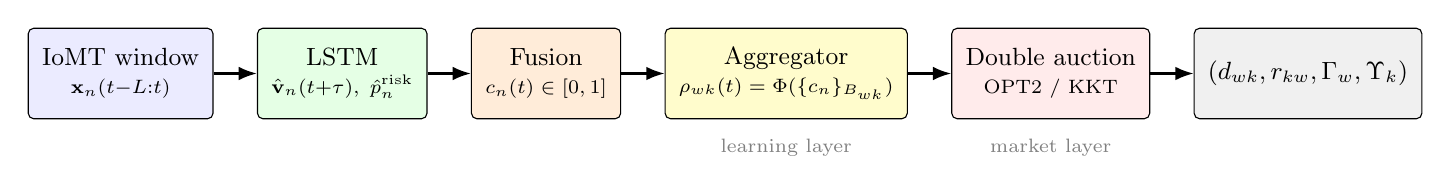
\begin{tikzpicture}[
  font=\small,
  box/.style={draw, rounded corners=2pt, align=center, inner sep=5pt, minimum height=1.15cm},
  arr/.style={-{Latex}, thick}
]
  \node[box, fill=blue!8] (iomt) {IoMT window\\[-1pt]{\scriptsize $\mathbf{x}_n(t{-}L{:}t)$}};
  \node[box, fill=green!10, right=0.55cm of iomt] (lstm) {LSTM\\[-1pt]{\scriptsize $\hat{\mathbf{v}}_n(t{+}\tau),\;\hat{p}_n^{\mathrm{risk}}$}};
  \node[box, fill=orange!15, right=0.55cm of lstm] (fuse) {Fusion\\[-1pt]{\scriptsize $c_n(t)\in[0,1]$}};
  \node[box, fill=yellow!20, right=0.55cm of fuse] (agg) {Aggregator\\[-1pt]{\scriptsize $\rho_{wk}(t)=\Phi(\{c_n\}_{B_{wk}})$}};
  \node[box, fill=red!8, right=0.55cm of agg] (auc) {Double auction\\[-1pt]{\scriptsize OPT2 / KKT}};
  \node[box, fill=gray!12, right=0.55cm of auc] (out) {$(d_{wk},r_{kw},\Gamma_w,\Upsilon_k)$};
  \draw[arr] (iomt) -- (lstm);
  \draw[arr] (lstm) -- (fuse);
  \draw[arr] (fuse) -- (agg);
  \draw[arr] (agg) -- (auc);
  \draw[arr] (auc) -- (out);
  \node[font=\scriptsize, gray, below=0.12cm of agg] {learning layer};
  \node[font=\scriptsize, gray, below=0.12cm of auc] {market layer};
\end{tikzpicture}
\caption{Double-auction market layer together with the learning layer that supplies a time-varying private preference \(\rho_{wk}(t)\) from IoMT forecasts. Reluctance \(\omega_{kw}\) is a constant per-cell table on this topology.}
\label{fig:pipeline}
\end{figure*}

\section{LSTM-Driven Preference}
\label{sec:lstm}

The path from vitals to preference is: bidirectional LSTM \(\to\) per-user criticality \(c_n\) \(\to\) coverage set \(B_{wk}\) \(\to\) preference \(\rho_{wk}\). This section writes that path as the maps used in the prototype.

\subsection{From bedside numerics to sequences}
Public tabular IoMT dumps are often cross-sectional. We therefore do \emph{not} synthesize AR(1) traces. The encoder is trained on the open eICU Collaborative Research Database Demo v2.0.1~\cite{pollard2018eicu,johnson2021eicudemo}: \(N=1821\) ICU stays with native \(5\)-minute medians from \texttt{vitalPeriodic} and non-invasive blood pressure from \texttt{vitalAperiodic}. A lookback of \(L=30\) steps (\(150\)\,min) yields a window \(\mathbf{x}_n\in\R^{L\times F}\), \(F=6\) (HR, SpO\(_2\), SBP, DBP, temperature, fall). Targets are the five vitals and a three-class NEWS2-style risk label at horizons \(\tau\in\{5,10,15\}\)\,min. Train / val / test are split \emph{by stay} (\(1274/273/274\)) so that no identity leaks; windows number \(52{,}159/11{,}186/11{,}109\). Vitals are standardized with a scaler fit on train stays only. We cite the Demo corpus honestly; this is not the credentialed full eICU-CRD.

\subsection{Multi-task bidirectional LSTM}
A two-layer bidirectional LSTM (hidden size \(128\), dropout \(0.25\)) emits a sequence of encodings \(\mathbf{h}_{n,1:L}\in\R^{L\times 256}\). Tanh attention pooling
\begin{equation}
  \alpha_{n,\ell}
  =\mathrm{softmax}_\ell\bigl(\mathbf{u}^\top\tanh(W\mathbf{h}_{n,\ell})\bigr),\qquad
  \mathbf{z}_n
  =\sum_{\ell=1}^{L}\alpha_{n,\ell}\,\mathbf{h}_{n,\ell}
  \label{eq:attn}
\end{equation}
produces a context vector. Two heads emit
\begin{align}
  \hat{\mathbf{V}}_n &\in\R^{3\times 5}
  &&\text{(vitals at three horizons),}\\
  \hat{\mathbf{P}}_n &\in\Delta^2
  &&\text{(softmax over }\{\text{normal, moderate, critical}\}\text{).}
\end{align}
Training minimizes Smooth-L1 on vitals plus class-weighted cross-entropy on risk,
\begin{equation}
  \mathcal{L}
  =\mathcal{L}_{\mathrm{vital}}
  +0.35\,\mathcal{L}_{\mathrm{risk}},
  \label{eq:lstm-loss}
\end{equation}
with Adam (\(\mathrm{lr}=10^{-3}\), weight decay \(10^{-4}\)), batch size \(256\), at most \(25\) epochs, gradient clip \(1.0\), and early stopping patience \(5\).

\subsection{Fusion: \(c_n\in[0,1]\)}
\label{sec:fusion}
Each predicted vital is mapped through a piecewise-linear NEWS2 band~\cite{royal2017news2} to a channel score in \([0,1]\). For a two-sided vital with inner (normal) interval \([a,b]\) and outer (critical) interval \([A,B]\),
\begin{equation}
  s(x;a,b,A,B)
  =
  \max\Bigl(
    \mathrm{clip}\tfrac{a-x}{a-A},\;
    \mathrm{clip}\tfrac{x-b}{B-b}
  \Bigr),
  \label{eq:band}
\end{equation}
with \(\mathrm{clip}(u)=\min(\max(u,0),1)\). SpO\(_2\) is one-sided (only hypoxemia is penalized):
\begin{equation}
  s_{\mathrm{SpO_2}}(x)=\mathrm{clip}\tfrac{96-x}{96-88}.
  \label{eq:spo2}
\end{equation}
The bands used in the prototype are listed in Table~\ref{tab:bands}. The LSTM risk head is collapsed to
\begin{equation}
  s_{\mathrm{risk}}
  = P(\mathrm{critical})+\tfrac12 P(\mathrm{moderate}).
  \label{eq:risk-head}
\end{equation}
Let \(\alpha_m\) be the channel weights in Table~\ref{tab:weights} (\(\sum_m\alpha_m=1\)). The per-horizon score of user \(n\) is
\begin{equation}
  s_n(\tau)
  =\sum_{m}\alpha_m\,s_{n,m}(\tau).
  \label{eq:channel-fuse}
\end{equation}
Horizon fusion mixes a recency-weighted mean with a peak term so a crash that is still \(15\) minutes away already lifts the score:
\begin{equation}
  c_n
  =
  \pi\,\max_{\tau}s_n(\tau)
  +(1-\pi)\sum_{\tau}w_{\tau}\,s_n(\tau),
  \label{eq:cn}
\end{equation}
with \((w_{5},w_{10},w_{15})=(0.50,0.30,0.20)\) and peak mix \(\pi=0.40\). The result is clipped to \([0,1]\).

\begin{table}[!t]
\caption{NEWS2-inspired vital bands used in~\eqref{eq:band}--\eqref{eq:spo2}.}
\label{tab:bands}
\centering
\begin{tabular}{@{}lcccc@{}}
\toprule
Channel & Inner low \(a\) & Inner high \(b\) & Outer low \(A\) & Outer high \(B\) \\
\midrule
HR (min\(^{-1}\)) & \(51\) & \(90\) & \(40\) & \(131\) \\
SpO\(_2\) (\%) & \(96\) & --- & \(88\) & --- \\
SBP (mmHg) & \(111\) & \(219\) & \(90\) & \(220\) \\
DBP (mmHg) & \(60\) & \(90\) & \(40\) & \(120\) \\
Temp (\(^\circ\)C) & \(36.1\) & \(38.0\) & \(35.0\) & \(39.1\) \\
\bottomrule
\end{tabular}
\end{table}

\begin{table}[!t]
\caption{Fusion channel weights (\(\sum\alpha_m=1\)) and horizon mix.}
\label{tab:weights}
\centering
\begin{tabular}{@{}lc@{\hspace{1.4em}}lc@{}}
\toprule
Channel & \(\alpha_m\) & Horizon term & Value \\
\midrule
SpO\(_2\) & \(0.26\) & \(w_5\) & \(0.50\) \\
SBP & \(0.18\) & \(w_{10}\) & \(0.30\) \\
HR & \(0.16\) & \(w_{15}\) & \(0.20\) \\
Fall & \(0.12\) & peak mix \(\pi\) & \(0.40\) \\
DBP & \(0.10\) & & \\
Risk head~\eqref{eq:risk-head} & \(0.10\) & & \\
Temperature & \(0.08\) & & \\
\bottomrule
\end{tabular}
\end{table}

\subsection{Aggregation to \(\rho_{wk}\)}
Users are placed uniformly in a \(2\,\mathrm{km}\times 2\,\mathrm{km}\) urban-micro layout. Association is max-RSRP under a 3GPP UMi-street NLOS-style path loss at \(3.5\,\mathrm{GHz}\)~\cite{3gppumi} with equal TX power \(30\,\mathrm{dBm}\):
\begin{equation}
  \mathrm{PL}(d)_{\mathrm{dB}}
  =32.4+20\log_{10}(f_c)+31.9\log_{10}(d),\qquad f_c=3.5.
  \label{eq:pl}
\end{equation}
Users are assigned independently and uniformly at random to one of \(W=2\) competing HSPs (HSP1, HSP2). This is a buyer label, not a clinical specialty: eICU stays have no hospital-of-record field, so disease names such as emergency or cardiology are not used. The assignment instantiates the coverage sets \(B_{wk}\). Write
\begin{equation}
  C_{wk}=\sum_{n\in B_{wk}} c_n,\qquad
  \bar c_{wk}=\frac{C_{wk}}{\lvert B_{wk}\rvert},\qquad
  \bar C=\frac{1}{WK}\sum_{w,k}C_{wk}.
  \label{eq:Cwk}
\end{equation}
The working preference used in experiments is the mass-scaled intensity, then max-normalized into \((0,1]\):
\begin{equation}
  \rho_{wk}^{\mathrm{raw}}
  =\frac{C_{wk}}{\bar C}\bigl(1+\bar c_{wk}\bigr),\qquad
  \rho_{wk}
  =\frac{\rho_{wk}^{\mathrm{raw}}}{\max_{w',k'}\rho_{w'k'}^{\mathrm{raw}}},
  \label{eq:rho-impl}
\end{equation}
with a floor \(\varepsilon=10^{-9}\) on empty links so that OPT2 logarithms remain defined. Equation~\eqref{eq:rho-impl} makes two effects explicit: \emph{mass} (many moderately sick users under a cell still raise demand) and \emph{intensity} (a few crashing users raise it too). Max-normalization keeps \(\rho_{wk}\in(0,1]\) as required by the theory text while preserving ranking.

\subsection{Clearing check}
To verify that a larger \(\rho_{wk}\) indeed buys more rate, we instantiate OPT1 with
\begin{equation}
  S_w=\sum_k \rho_{wk}\log(1+h_{wk}d_{wk}),
  \quad
  T_k=\sum_w \omega_{kw}\Bigl(c r_{kw}+\tfrac{\beta}{2}r_{kw}^2\Bigr),
  \label{eq:impl-util}
\end{equation}
which satisfy~\eqref{eq:hsp-shape}--\eqref{eq:bs-shape}. Channel quality is a scaled relative gain \(h_{wk}=10\cdot g_{wk}/\max g\). We solve the KKT system by nested bisection on \((\lambda,\mu)\) plus a sub-gradient on a link price \(\pi_{wk}\) until \(d_{wk}\approx r_{kw}\). Cleared rate and payment on a link are
\begin{equation}
  x_{wk}=\tfrac12(d_{wk}+r_{kw}),\qquad
  P_{wk}=\pi_{wk}\,x_{wk}.
  \label{eq:x-pay}
\end{equation}
The truthful BS bid implied by~\eqref{eq:impl-util} is \(\zeta_{kw}=\omega_{kw}(c/r_{kw}+\beta)\). This solver is a \emph{centralized} cousin of OPT2, used only as an empirical probe; the deployable protocol remains the dual iteration of Section~\ref{sec:base}.

\section{Constant Reluctance}
\label{sec:omega-impl}

Section~\ref{sec:base} parameterizes BS cost by a reluctance \(\omega_{kw}\in[0,1]\). This paper holds \(\omega\) \emph{constant}: the same value throughout the inner dual loop and throughout the reported experiment. Preference is the dynamic object; reluctance is a fixed per-cell cost scale on the \(3\times 2\) topology.

eICU has bedside numerics, not operator RAN counters. We evaluate a closed-form logistic once on the association geometry,
\begin{equation}
  \omega_{kw}^{\star}
  =\sigma\bigl(\mathbf{a}^\top\boldsymbol{\xi}_{kw}+b\bigr),\qquad
  \sigma(z)=\bigl(1+e^{-z}\bigr)^{-1},
  \label{eq:omega-star}
\end{equation}
with features \(\boldsymbol{\xi}=(\eta,\bar\gamma,b,q^{\mathrm{nat}},I)\) (cell load, mean RSRP quality, backhaul, native-user QoS degradation, interference) and
\begin{equation}
  \mathbf{a}=(1.35,\,-1.55,\,0.95,\,1.05,\,0.90),\qquad b=-0.85.
  \label{eq:omega-ab}
\end{equation}
Load, backhaul, native QoS and interference are cell-level, so both HSPs see essentially the same \(\omega\) under a given BS. Table~\ref{tab:omega-const} is the frozen matrix consumed by the auction (Fig.~\ref{fig:omega-const}). Rows match because reluctance is a property of the cell, not of a hospital specialty. The honest claim is: \emph{dynamic preference from real ICU numerics; constant reluctance from one radio-geometry snapshot on the same map.}

\begin{table}[!t]
\caption{Frozen reluctance \(\omega_{kw}\) on the \(W=2\), \(K=3\) map. Rows are nearly identical because \(\omega\) is evaluated once per cell.}
\label{tab:omega-const}
\centering
\begin{tabular}{@{}lccc@{}}
\toprule
HSP \(w\) \(\backslash\) BS \(k\) & \(1\) & \(2\) & \(3\) \\
\midrule
HSP1  & \(0.390\) & \(0.562\) & \(0.559\) \\
HSP2  & \(0.390\) & \(0.563\) & \(0.559\) \\
\bottomrule
\end{tabular}
\end{table}

\begin{figure}[!t]
\centering

\includegraphics[width=0.78\linewidth]{fig_omega_const.png}
\caption{Constant reluctance \(\omega_{kw}\) from the one-shot radio-geometry map. HSP1 and HSP2 share a cell's value.}
\label{fig:omega-const}
\end{figure}

\section{Experimental Setup}
\label{sec:setup}

Unless noted, every number in Section~\ref{sec:results} is generated with the constants in Tables~\ref{tab:bands}--\ref{tab:learn}. Paper indices are \(w=\)HSP, \(k=\)BS. Implementation arrays are stored as \((\mathrm{BS},\mathrm{HSP})\) and are transposed in every table below. HSP1 and HSP2 are two randomly assigned competing buyers. BS1 is the first site in the layout (code index \(0\)).

\begin{table}[!t]
\caption{Market, radio, and auction constants (static unless marked *).}
\label{tab:auction}
\centering
\begin{tabular}{@{}lll@{}}
\toprule
Symbol & Meaning & Value \\
\midrule
\(W,K\) & HSPs, BSs (this experiment) & \(2,\;3\) \\
\(r^{\max}\) & BS capacity (uniform) & \(5\) Mbps \\
over-subscription & HSP demand cap vs.\ supply & \(1.20\) \\
\(c\) & linear OPEX & \(0.03\) \\
\(\beta\) & quadratic congestion & \(0.015\) \\
\(h\) scale & \(h_{wk}=10\,g_{wk}/\max g\) & \(10\) \\
\(\Delta_0\) & sub-gradient step & \(0.04/\sqrt{t}\) \\
tol, max iter. & clearing gap / cap & \(10^{-3}\), \(600\) \\
map, \(f_c\), \(P_{\mathrm{tx}}\) & UMi layout & \(2\,\mathrm{km}\), \(3.5\,\mathrm{GHz}\), \(30\,\mathrm{dBm}\) \\
HSP assignment & competing buyers & random, seed \(42\) \\
seed & RNG & \(42\) \\
\bottomrule
\end{tabular}
\end{table}

\begin{table}[!t]
\caption{Learning-layer constants (static). Fusion weights are in Table~\ref{tab:weights}.}
\label{tab:learn}
\centering
\begin{tabular}{@{}lll@{}}
\toprule
Symbol / name & Meaning & Value \\
\midrule
corpus & vitals source & eICU-CRD Demo v2.0.1 \\
\(N_{\mathrm{stay}}\) & ICU stays & \(1821\) \\
windows & train / val / test & \(52{,}159/11{,}186/11{,}109\) \\
\(L\), stride & lookback / window stride & \(30\) steps (\(150\)\,min), \(30\)\,min \\
\(\tau\) & forecast horizons & \(5,10,15\)\,min \\
BiLSTM & layers, hidden, dropout & \(2\), \(128\), \(0.25\) \\
Adam & lr, weight decay, batch & \(10^{-3}\), \(10^{-4}\), \(256\) \\
epochs, patience, clip & training & \(25\), \(5\), \(1.0\) \\
\(\mathcal{L}\) & loss mix~\eqref{eq:lstm-loss} & Smooth-L1 \(+0.35\) CE \\
\(\mathbf{a},b\) & \(\omega^\star\) logistic~\eqref{eq:omega-ab} & \((1.35,-1.55,0.95,1.05,0.90)\), \(-0.85\) \\
\(\omega\) & held constant (Table~\ref{tab:omega-const}) & one radio snapshot \\
\bottomrule
\end{tabular}
\end{table}

\section{Experimental Results}
\label{sec:results}

All matrices below are \(W\times K\) in paper order: rows are HSP1 and HSP2; columns are BS1, BS2, BS3.

\subsection{Forecast quality}
Held-out test performance is summarized in Table~\ref{tab:lstm} and Figs.~\ref{fig:lstm-train}--\ref{fig:lstm-mae}. Overall vital MAE is \(2.28\) (mixed clinical units), risk accuracy \(80.7\%\), macro-F1 \(0.723\). Accuracy declines mildly from \(5\) to \(15\)\,min (\(84.1\%\to 77.6\%\)), which is expected on real ICU traces and still usable for a \(15\)-minute look-ahead preference.

\begin{figure}[!t]
\centering

\includegraphics[width=0.98\linewidth]{fig_lstm_training.png}
\caption{LSTM training and validation loss, and risk-head accuracy, over epochs.}
\label{fig:lstm-train}
\end{figure}

\begin{figure}[!t]
\centering

\includegraphics[width=0.98\linewidth]{fig_lstm_mae.png}
\caption{Test vital MAE by horizon on the eICU-CRD Demo hold-out.}
\label{fig:lstm-mae}
\end{figure}

\begin{table}[!t]
\caption{Bidirectional LSTM test metrics on eICU-CRD Demo (11{,}109 windows). MAE in clinical units.}
\label{tab:lstm}
\centering
\begin{tabular}{@{}lcccccc@{}}
\toprule
Horizon & HR & SpO\(_2\) & SBP & DBP & Temp & Risk acc. \\
\midrule
\(5\) min  & \(2.41\) & \(0.79\) & \(3.18\) & \(2.34\) & \(0.009\) & \(84.1\%\) \\
\(10\) min & \(2.95\) & \(0.95\) & \(4.53\) & \(3.30\) & \(0.009\) & \(80.4\%\) \\
\(15\) min & \(3.31\) & \(1.10\) & \(5.34\) & \(3.89\) & \(0.010\) & \(77.6\%\) \\
\bottomrule
\end{tabular}
\end{table}

\subsection{Fused criticality}
On \(74{,}454\) windows, \(c_n\in[0.0004,0.753]\) with mean \(0.115\) (median \(0.087\)). Mean \(c_n\) increases with a snapshot-risk label that was \emph{not} an input to fusion: \(0.075\) (normal), \(0.139\) (moderate), \(0.218\) (critical). The ranking is milder than a synthetic disease cartoon: eICU Demo mixes real ICU phenotypes, so heart-disease and respiratory-failure stays sit only modestly above hypertension and trauma (Table~\ref{tab:cn}).

\begin{table}[!t]
\caption{Fused criticality \(c_n\) on eICU-CRD Demo windows.}
\label{tab:cn}
\centering
\begin{tabular}{@{}lc@{\hspace{1.2em}}lc@{}}
\toprule
Snapshot risk & Mean \(c_n\) & Disease & Mean \(c_n\) \\
\midrule
0 (normal)    & \(0.075\) & Heart disease        & \(0.127\) \\
1 (moderate)  & \(0.139\) & Respiratory failure  & \(0.125\) \\
2 (critical)  & \(0.218\) & Diabetes mellitus    & \(0.103\) \\
              &           & General              & \(0.110\) \\
              &           & Hypertension         & \(0.088\) \\
\bottomrule
\end{tabular}
\end{table}

\subsection{Coverage, mass, and preference (\(3\times 2\) market)}
Every link is populated. Table~\ref{tab:Nwk} counts users; Table~\ref{tab:Cwk} is the criticality mass \(C_{wk}\) of~\eqref{eq:Cwk}; Table~\ref{tab:cbar} is the mean intensity \(\bar c_{wk}\); Table~\ref{tab:rho} is the max-normalized preference~\eqref{eq:rho-impl}. The random split is balanced (about \(37.2\)k users per HSP). Preference therefore ranks cells by coverage, not by a clinical specialty: BS2/BS3 sit above BS1 because those cells cover more of the map (Fig.~\ref{fig:pref-anatomy}). Raising one HSP's \(\rho\) raises both its rate and its payment (Fig.~\ref{fig:pref-pay}).

\begin{table}[!t]
\caption{Coverage count \(\lvert B_{wk}\rvert\).}
\label{tab:Nwk}
\centering
\begin{tabular}{@{}lccc@{}}
\toprule
HSP \(w\) \(\backslash\) BS \(k\) & \(1\) & \(2\) & \(3\) \\
\midrule
HSP1  & \(9220\) & \(13902\) & \(14053\) \\
HSP2  & \(9379\) & \(13962\) & \(13938\) \\
\bottomrule
\end{tabular}
\end{table}

\begin{table}[!t]
\caption{Criticality mass \(C_{wk}=\sum_{n\in B_{wk}}c_n\).}
\label{tab:Cwk}
\centering
\begin{tabular}{@{}lccc@{}}
\toprule
HSP \(w\) \(\backslash\) BS \(k\) & \(1\) & \(2\) & \(3\) \\
\midrule
HSP1  & \(1076.57\) & \(1594.91\) & \(1611.72\) \\
HSP2  & \(1070.79\) & \(1620.54\) & \(1605.79\) \\
\bottomrule
\end{tabular}
\end{table}

\begin{table}[!t]
\caption{Mean per-user criticality \(\bar c_{wk}\).}
\label{tab:cbar}
\centering
\begin{tabular}{@{}lccc@{}}
\toprule
HSP \(w\) \(\backslash\) BS \(k\) & \(1\) & \(2\) & \(3\) \\
\midrule
HSP1  & \(0.117\) & \(0.115\) & \(0.115\) \\
HSP2  & \(0.114\) & \(0.116\) & \(0.115\) \\
\bottomrule
\end{tabular}
\end{table}

\begin{table}[!t]
\caption{Max-normalized preference \(\rho_{wk}\) from~\eqref{eq:rho-impl} (one slot; largest entry \(1\)).}
\label{tab:rho}
\centering
\begin{tabular}{@{}lccc@{}}
\toprule
HSP \(w\) \(\backslash\) BS \(k\) & \(1\) & \(2\) & \(3\) \\
\midrule
HSP1  & \(0.665\) & \(0.983\) & \(0.993\) \\
HSP2  & \(0.660\) & \(1.000\) & \(0.990\) \\
\bottomrule
\end{tabular}
\end{table}

\begin{figure*}[!t]
\centering

\includegraphics[width=0.98\linewidth]{fig6_preference_criticality.png}
\caption{Criticality mass \(C_{wk}\), mean per-user criticality \(\bar c_{wk}\), and preference \(\rho_{wk}\) of each HSP toward the three BSs (\(W=2\), \(K=3\)).}
\label{fig:pref-anatomy}
\end{figure*}

\begin{figure*}[!t]
\centering

\includegraphics[width=0.98\linewidth]{fig8_preference_vs_payment.png}
\caption{Preference versus cleared rate and payment, and comparative statics in a scale \(\alpha\) applied to one HSP's \(\rho\).}
\label{fig:pref-pay}
\end{figure*}

\subsection{Auction follows preference under constant reluctance}
A single one-slot clearing uses the \(\rho_{wk}\) of Table~\ref{tab:rho} and the frozen \(\omega_{kw}\) of Table~\ref{tab:omega-const}. Each cell has \(r_k^{\max}=5\)\,Mbps (no load scaling). The market converges in \(226\) dual steps to welfare \(10.65\), total rate \(15.01\)\,Mbps, and payment \(4.37\), with gap \(9.95\times 10^{-4}\) (Table~\ref{tab:macro}). Seller capacity duals are positive on every cell, so the PRB cap binds; buyer demand caps remain slack. Over-subscription \(1.2\) keeps the HSP-side demand envelope at \(1.2\times 15=18\)\,Mbps.

The two buyers have nearly identical preference after the random split. Allocation differences therefore come from geometry (who sits in \(B_{wk}\) and the resulting channel gain), not from a clinical specialty label. HSP1 is allocated \(8.40\)\,Mbps and HSP2 \(6.61\)\,Mbps (Table~\ref{tab:rates-d}). All buyer surpluses and seller profits stay positive (Table~\ref{tab:surplus}).

Fig.~\ref{fig:conv} shows that the dual iteration on this frozen-\(\omega\) market converges for step sizes \(\Delta\in\{0.04,0.06\}\); \(\Delta=0.02\) is still gappy at \(250\) iterations under the tight \(5\)\,Mbps cap. Fig.~\ref{fig:gap} is the per-link demand--response gap; Figs.~\ref{fig:bs-bids} and~\ref{fig:hsp-bids} are the implied BS and HSP bids. Fig.~\ref{fig:pay-surplus} records HSP outlay, BS receipt, buyer surplus and seller profit. A GBDT predictor and a stressed-cell experiment exist in the code tree; they are \emph{not} paper-1 claims.

\begin{table}[!t]
\caption{Macro clearing on the \(W=2\), \(K=3\) market (\(r_k^{\max}=5\)\,Mbps, frozen \(\omega\)).}
\label{tab:macro}
\centering
\begin{tabular}{@{}lcccc@{}}
\toprule
Setting & SW & Rate (Mbps) & Payment & Gap \\
\midrule
Frozen \(\omega\) & \(10.65\) & \(15.01\) & \(4.37\) & \(9.95\times 10^{-4}\) \\
\bottomrule
\end{tabular}
\end{table}

\begin{figure}[!t]
\centering

\includegraphics[width=0.98\linewidth]{fig2_convergence.png}
\caption{Convergence of social welfare under frozen reluctance for step sizes \(\Delta\in\{0.02,0.04,0.06\}\).}
\label{fig:conv}
\end{figure}

\begin{figure*}[!t]
\centering

\includegraphics[width=0.98\linewidth]{fig3_demand_response_gap_all.png}
\caption{Demand--response gap \(d_{wk}-r_{kw}\) on every (HSP, BS) link (\(\Delta=0.04\)).}
\label{fig:gap}
\end{figure*}

\begin{figure*}[!t]
\centering

\includegraphics[width=0.98\linewidth]{fig4_bs_bids.png}
\caption{Evolution of BS bids \(\zeta_{kw}\) (\(\Delta=0.04\)).}
\label{fig:bs-bids}
\end{figure*}

\begin{figure*}[!t]
\centering

\includegraphics[width=0.98\linewidth]{fig5_hsp_bids.png}
\caption{Evolution of HSP bids \(\varrho_{wk}\) (\(\Delta=0.04\)).}
\label{fig:hsp-bids}
\end{figure*}

\begin{figure*}[!t]
\centering

\includegraphics[width=0.98\linewidth]{fig7_payments_surplus.png}
\caption{HSP outlay versus BS receipt, and buyer surplus versus seller profit, under frozen \(\omega\).}
\label{fig:pay-surplus}
\end{figure*}

\begin{table}[!t]
\caption{Cleared uplink \(x_{wk}\) (Mbps) under frozen \(\omega\).}
\label{tab:rates-d}
\centering
\begin{tabular}{@{}lccc@{}}
\toprule
HSP \(w\) \(\backslash\) BS \(k\) & \(1\) & \(2\) & \(3\) \\
\midrule
HSP1  & \(2.886\) & \(2.917\) & \(2.598\) \\
HSP2  & \(2.114\) & \(2.084\) & \(2.410\) \\
\bottomrule
\end{tabular}
\end{table}

\begin{table}[!t]
\caption{Link payment \(P_{wk}=\pi_{wk}x_{wk}\) under frozen \(\omega\).}
\label{tab:pay-d}
\centering
\begin{tabular}{@{}lccc@{}}
\toprule
HSP \(w\) \(\backslash\) BS \(k\) & \(1\) & \(2\) & \(3\) \\
\midrule
HSP1  & \(0.642\) & \(0.860\) & \(0.940\) \\
HSP2  & \(0.461\) & \(0.600\) & \(0.868\) \\
\bottomrule
\end{tabular}
\end{table}

\begin{table}[!t]
\caption{Buyer surplus and seller profit under frozen \(\omega\).}
\label{tab:surplus}
\centering
\begin{tabular}{@{}lc@{}}
\toprule
Agent & Value \\
\midrule
HSP1 surplus & \(4.79\) \\
HSP2 surplus & \(1.86\) \\
BS1 profit & \(1.01\) \\
BS2 profit & \(1.32\) \\
BS3 profit & \(1.67\) \\
\bottomrule
\end{tabular}
\end{table}

These numbers show that once \(\rho_{wk}\) is generated from predicted criticality and \(\omega_{kw}\) is held at the radio-geometry snapshot, the same concave program clears a capacity-binding \(5\)\,Mbps market with positive surplus on both sides.

\section{Further Extensions}
\label{sec:ext}

LSTM+fusion makes \(\rho_{wk}\) a function of \emph{time} and of \emph{who} sits in \(B_{wk}\). Reluctance is a constant table in this paper. Two structural facts of a 5G healthcare deployment are still ignored: spatial coupling of neighbouring cells, and a joint predictor that emits \((\rho,\omega)\) from one graph. Making \(\omega\) time-varying (or predicting it with a GBDT) is left to later work.

\subsection{GNN over the BS--HSP--user graph}
\label{sec:gnn}

\paragraph{Graph.}
Construct a tripartite graph \(\mathcal{G}=(V_U\cup V_W\cup V_K,E)\) at each slot \(t\):
\begin{itemize}
  \item user nodes \(n\in V_U\) with features \(\bigl(\mathbf{x}_n(t),\,c_n(t),\,\text{RSRP}\bigr)\);
  \item HSP nodes \(w\in V_W\) with features (subscriber count, cloud-backhaul headroom);
  \item BS nodes \(k\in V_K\) with features (PRB occupancy, native-user load, \(r_k^{\max}\), mean RSRP, neighbour interference).
\end{itemize}
Edges: user--BS if associated (or if RSRP is within a hand-off margin); user--HSP if subscribed; BS--HSP if \(B_{wk}\neq\emptyset\). Optional BS--BS edges encode co-channel interference.

\paragraph{Message passing.}
A stack of graph-attention layers~\cite{velickovic2018gat} (or GCN~\cite{kipf2017gcn}) updates
\begin{equation}
  \mathbf{z}_i^{(\ell+1)}
  =\mathrm{AGG}_{j\in\mathcal{N}(i)}
  \alpha_{ij}^{(\ell)}\,W^{(\ell)}\mathbf{z}_j^{(\ell)}.
\end{equation}
An edge head on each BS--HSP link emits
\begin{equation}
  \bigl(\hat\rho_{wk}(t),\,\hat\omega_{kw}(t)\bigr)
  =\psi\bigl(\mathbf{z}_w^{(L)}\,\Vert\,\mathbf{z}_k^{(L)}\,\Vert\,\mathbf{e}_{wk}\bigr),
  \label{eq:gnn-head}
\end{equation}
optionally constrained to \([0,1]\) by a sigmoid, matching the domain of \(\rho_{wk}\) and \(\omega_{kw}\) in Section~\ref{sec:base}.

\paragraph{Why a GNN rather than another LSTM.}
The LSTM already consumes the \emph{temporal} axis of each user. What it cannot see is that (i)~two BSs that share an interference neighbourhood should not independently ``accept'' the same critical burst, (ii)~an HSP whose subscribers straddle a hand-off boundary has a preference that is a \emph{smooth} function of two RSRP fields, and (iii)~reluctance at \(k\) depends on native load that is itself a function of neighbouring cells. Those are graph inductive biases. Training targets for \(\hat\rho_{wk}\) can be the aggregator~\eqref{eq:rho-impl}; targets for \(\hat\omega_{kw}\) can be the closed form~\eqref{eq:omega-star}. A self-supervised alternative is to train the GNN end-to-end so that the OPT1 welfare on \((\hat\rho,\hat\omega)\) matches a privileged simulator that sees future vitals and future SINR.

\paragraph{Interface to the auction.}
The GNN is evaluated \emph{privately}: HSP \(w\) runs (or is sent) the subgraph of its subscribers and produces \(\hat\rho_{w\cdot}(t)\); BS \(k\) produces \(\hat\omega_{k\cdot}(t)\). Bids~\eqref{eq:truthful-bids} are unchanged. The TPE still does not see the graph. The closed-form map~\eqref{eq:omega-star} already supplies a per-link \(\omega\); the GNN is the spatially coupled replacement, not a second independent reluctance model.

\paragraph{Joint dynamics.}
A complete slot-\(t\) update is
\begin{align}
  \{c_n(t)\}_n
    &\leftarrow \mathrm{LSTM{+}fusion}(\{\mathbf{x}_n(t)\}_n),
    \nonumber\\
  B_{wk}(t)
    &\leftarrow \text{association / hand-off},
    \nonumber\\
  \bigl(\rho_{wk}(t),\omega_{kw}(t)\bigr)
    &\leftarrow \mathrm{GNN}(\mathcal{G}_t),
    \label{eq:slot}\\
  (d_{wk}(t),r_{kw}(t),\Gamma_w,\Upsilon_k)
    &\leftarrow \text{dual iteration of Section~\ref{sec:base}}.
    \nonumber
\end{align}
Convergence theorems of the inner auction still apply \emph{conditional on} \((\rho(t),\omega(t))\), because those parameters are constant during the inner dual loop---the same modelling choice as a single shot of OPT1/OPT2. Across slots, \((\rho,\omega)\) form an exogenous (learned) process. Proving incentive compatibility when agents can \emph{manipulate the learning module} (e.g.\ an HSP spoofing vitals to inflate \(\rho\)) is an open problem; a practical mitigation is to compute \(c_n\) from authenticated device streams and to keep the GNN on the TPE's or the hospital's side of a TEE.

\subsection{Other natural extensions}
\begin{itemize}
  \item \emph{Online LSTM.} Replace one-shot windows by a stateful encoder that updates \(c_n\) every minute with \(O(1)\) hidden-state cost.
  \item \emph{Slice-aware OPT1.} Split \(d_{wk}\) into eMBB / URLLC components with separate \(\rho_{wk}^{\mathrm{eMBB}}\) and \(\rho_{wk}^{\mathrm{URLLC}}\) derived from different fusion horizons.
  \item \emph{Robustness.} Train the LSTM under missing-sensor and adversarial-noise models so that \(\rho_{wk}\) cannot be gamed by a single corrupted SpO\(_2\) stream.
  \item \emph{RL step-size.} Adapt the dual step \(\Delta\) by reinforcement learning. Combining that with dynamic \((\rho,\omega)\) yields a fully adaptive inner loop whose outer loop is the GNN.
\end{itemize}

\section{Conclusion}
\label{sec:conc}

We presented a double auction for 5G healthcare resource allocation that elicits private HSP utilities and BS costs and converges to the social-welfare KKT point without a central planner seeing either function. Preference \(\rho_{wk}\) is a forecast of criticality mass on a coverage set, implemented with a bidirectional LSTM, a NEWS2 fusion~\eqref{eq:cn}, and the max-normalized aggregator~\eqref{eq:rho-impl}. Reluctance is held constant: \(\omega^\star=\sigma(\mathbf{a}^\top\boldsymbol{\xi}+b)\) is evaluated once on the radio-geometry snapshot, and the BS cost is \(T=\omega(cr+\beta r^2/2)\). On the eICU-CRD Demo (\(N=1821\) stays) users are split at random into two competing buyers. With \(r_k^{\max}=5\)\,Mbps per cell the \(W=2\), \(K=3\) market clears at welfare \(10.65\) and total rate \(15.01\)\,Mbps; the LSTM attains test vital MAE \(2.28\) and risk accuracy \(80.7\%\). The TPE of this paper still sees cleartext bids; hiding those scalars (two-server HE or a TEE) is future work. A natural next market layer is a GNN on the user--HSP--BS graph that emits time-varying \((\rho_{wk}(t),\omega_{kw}(t))\) together from topology.

\appendices
\section{Notation Map}
\label{app:notation}
Table~\ref{tab:not} collects the notation used in this paper. Implementation arrays use the opposite index convention (first index BS); all numbers in Section~\ref{sec:results} have been transposed to \((w=\mathrm{HSP},\;k=\mathrm{BS})\).

\begin{table}[!t]
\caption{Notation (symbols marked * are introduced for the learning layer).}
\label{tab:not}
\centering
\begin{tabular}{@{}cl@{}}
\toprule
Symbol & Meaning \\
\midrule
\(w\in\mathcal{W}\) & HSP (buyer) \\
\(k\in\mathcal{K}\) & BS / CNP (seller) \\
\(B_{wk}\) & users of \(w\) under coverage of \(k\) \\
\(d_{wk},\;r_{kw}\) & requested / offered uplink rate \\
\(\rho_{wk}\) & HSP preference for BS \(k\) \\
\(\omega_{kw}\) & BS reluctance toward HSP \(w\) \\
\(\varrho_{wk},\;\zeta_{kw}\) & bids of HSP / BS \\
\(\lambda_k,\;\mu_{wk}\) & capacity / clearing duals \\
\(c_n(t)\) * & fused predicted criticality of user \(n\) \\
\(\Phi\) * & aggregator \(B_{wk}\mapsto\rho_{wk}(t)\) \\
\(\boldsymbol{\xi}_{kw}(t)\) * & physical features of reluctance \\
\bottomrule
\end{tabular}
\end{table}

\bibliographystyle{IEEEtran}
\bibliography{references}

\end{document}
